\chapter{Results}
\label{ch:results}


\section{Evolution of Patterns}


\subsection{Evolution of Encoded Variability}

\begin{figure}
  \begin{center}
    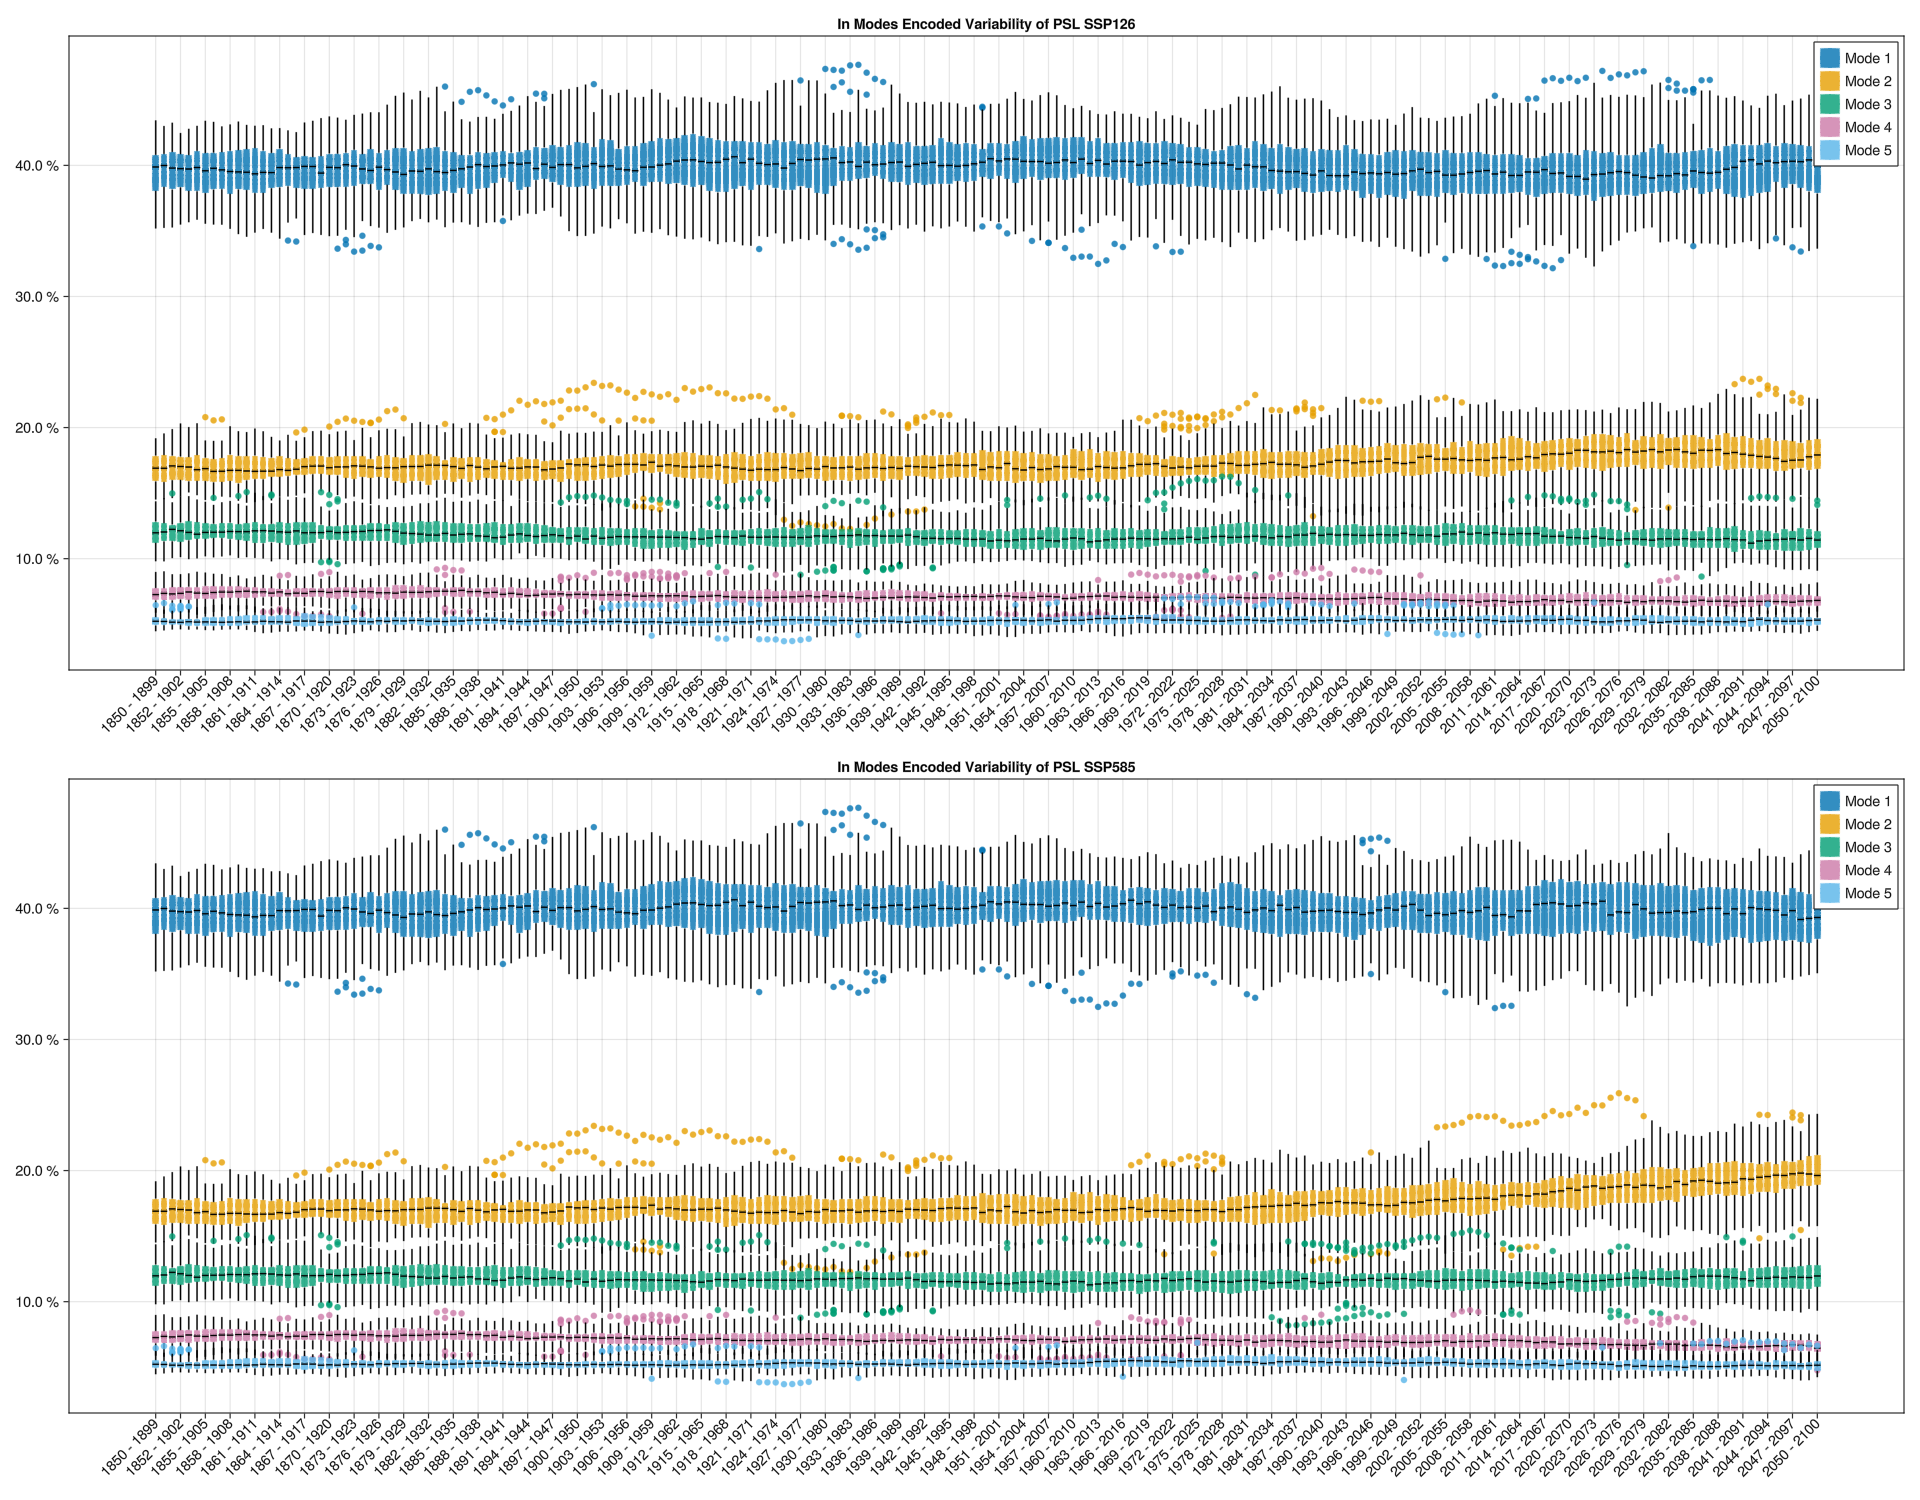
\includegraphics[width=0.95\textwidth]{figures/mode_variability_psl_50seasons.png}
  \end{center}
  \caption{Boxplot of the variability encoded in the top five modes of PSL EOF.}\label{fig:psl mode variability}
\end{figure}

\begin{figure}
  \begin{center}
    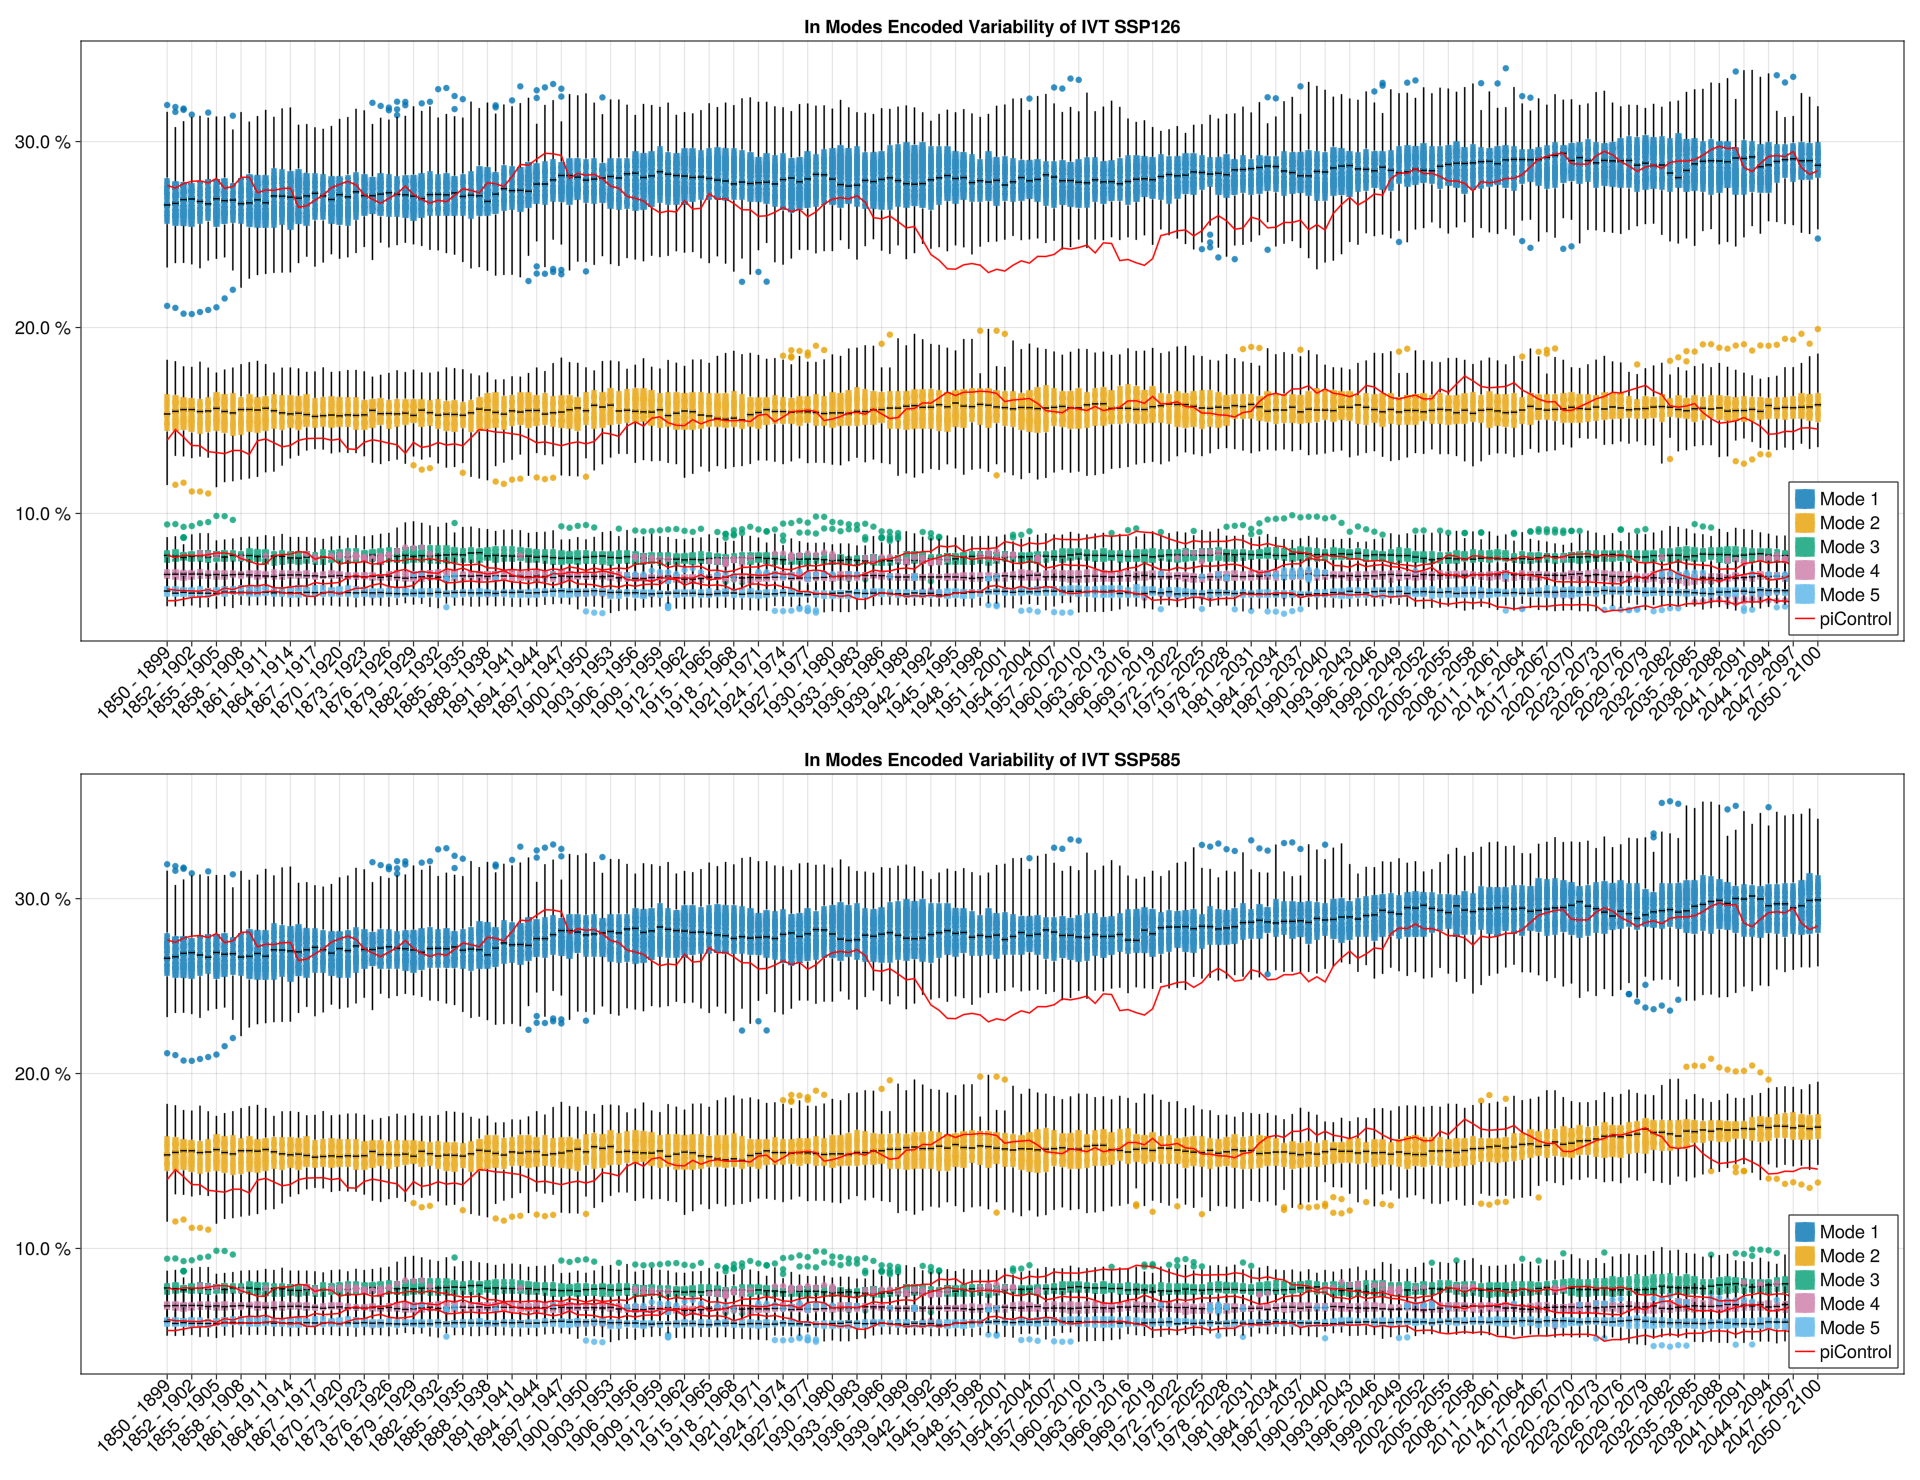
\includegraphics[width=0.95\textwidth]{figures/mode_variability_ivt_50seasons.png}
  \end{center}
  \caption{Same as Figure~\ref{fig:psl mode variability} but with IVT}\label{fig:ivt mode variability}
\end{figure}


\begin{figure}
  \begin{center}
    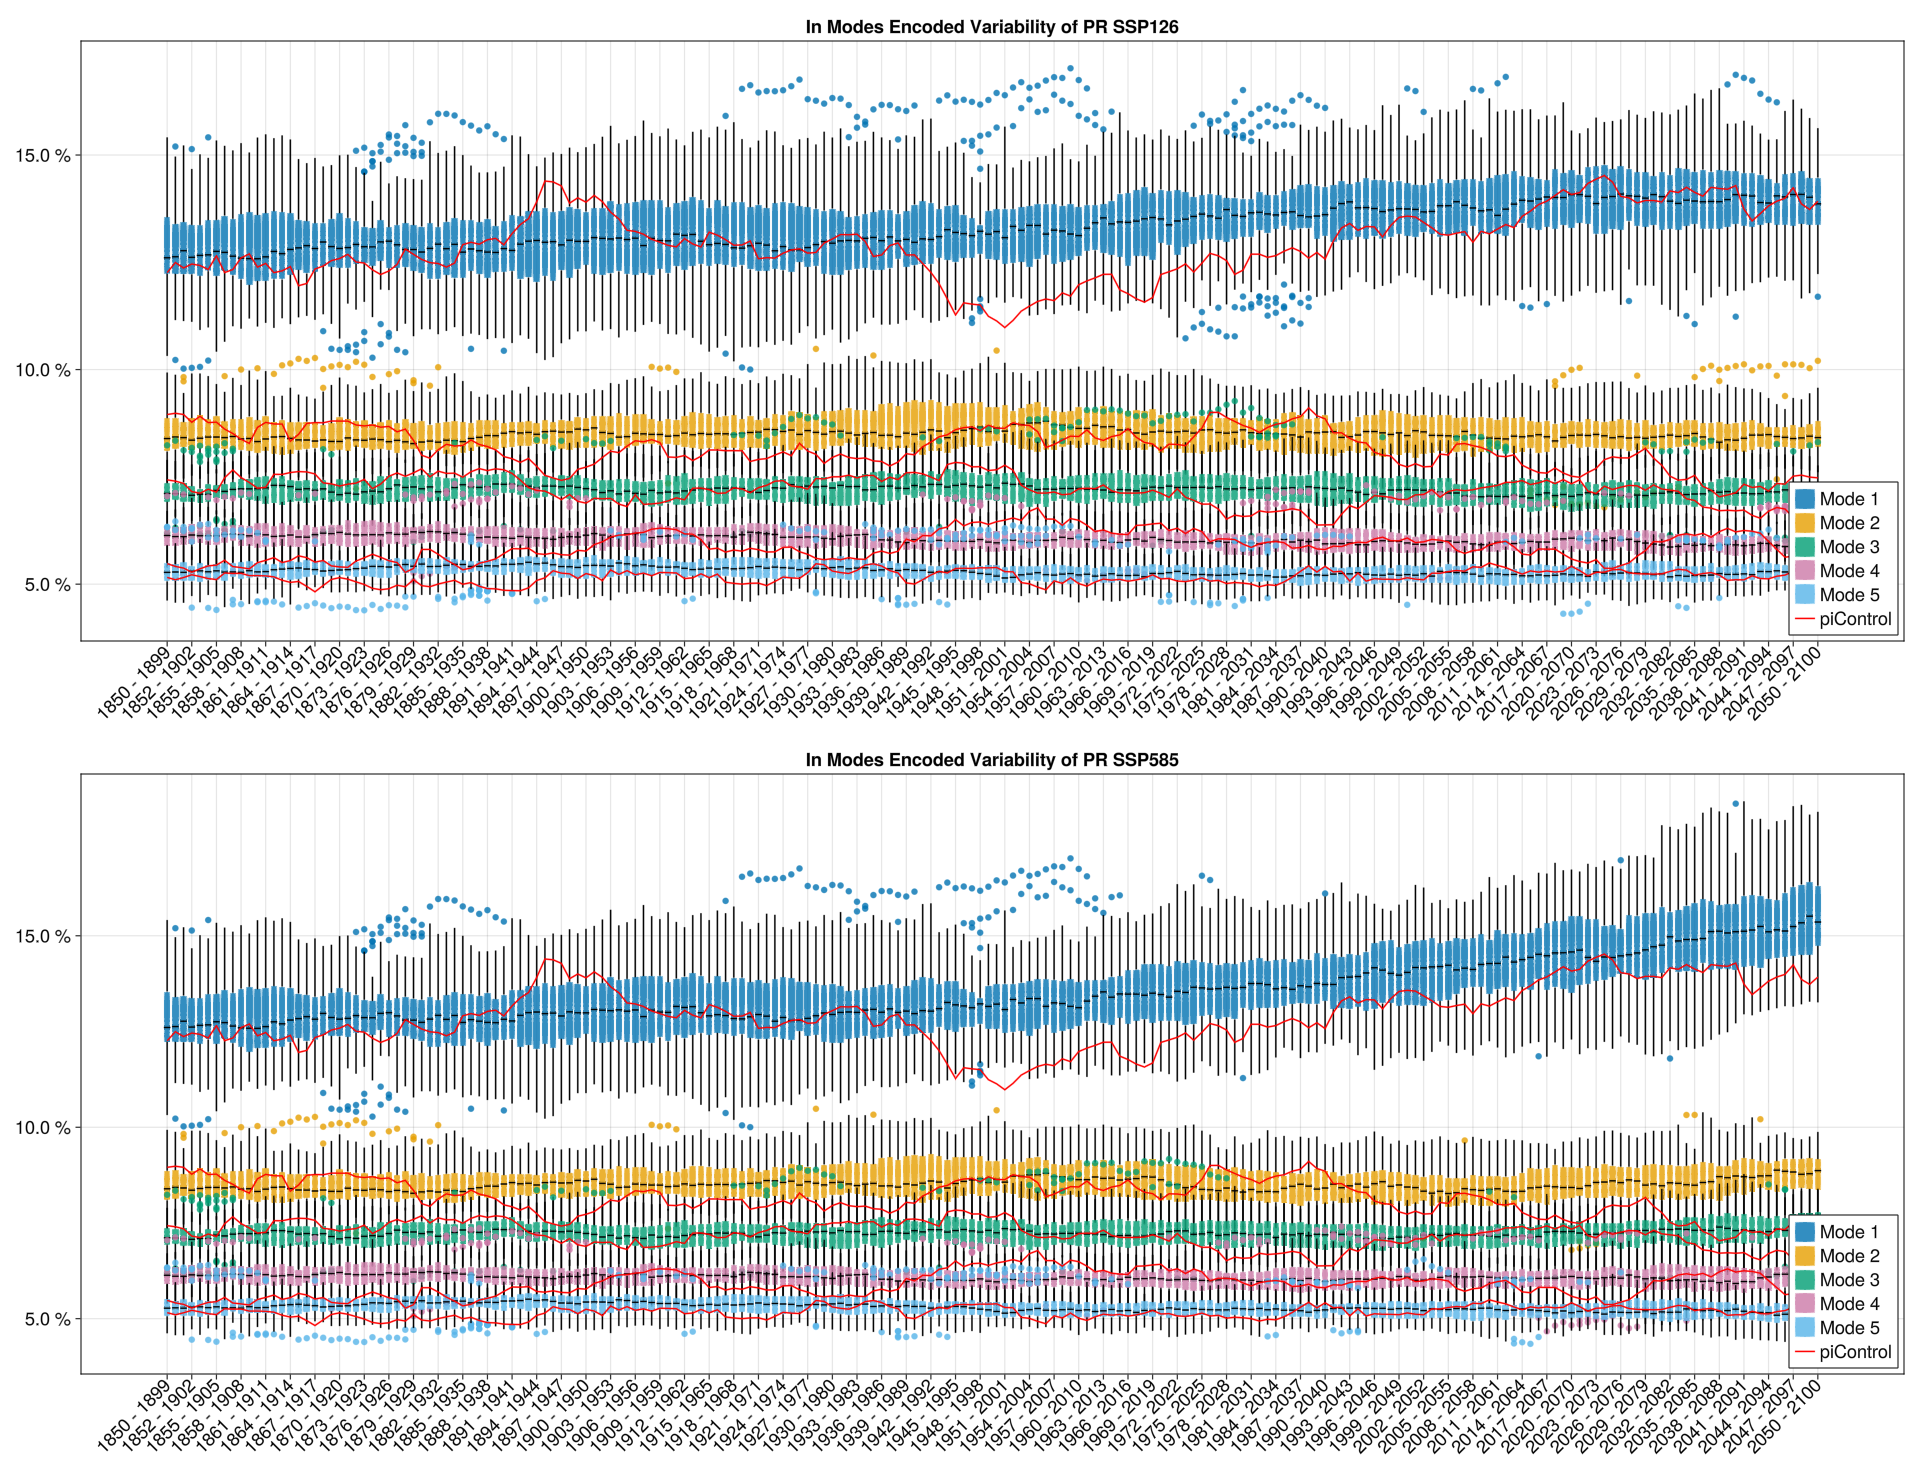
\includegraphics[width=0.95\textwidth]{figures/mode_variability_pr_50seasons.png}
  \end{center}
  \caption{Same as Figure~\ref{fig:psl mode variability} but with precipitation}\label{fig:pr mode variability}
\end{figure}
